%%
%% This is file `sample-sigconf-authordraft.tex',
%% generated with the docstrip utility.
%%
%% The original source files were:
%%
%% samples.dtx  (with options: `all,proceedings,bibtex,authordraft')
%% 
%% IMPORTANT NOTICE:
%% 
%% For the copyright see the source file.
%% 
%% Any modified versions of this file must be renamed
%% with new filenames distinct from sample-sigconf-authordraft.tex.
%% 
%% For distribution of the original source see the terms
%% for copying and modification in the file samples.dtx.
%% 
%% This generated file may be distributed as long as the
%% original source files, as listed above, are part of the
%% same distribution. (The sources need not necessarily be
%% in the same archive or directory.)
%%
%%
%% Commands for TeXCount
%TC:macro \cite [option:text,text]
%TC:macro \citep [option:text,text]
%TC:macro \citet [option:text,text]
%TC:envir table 0 1
%TC:envir table* 0 1
%TC:envir tabular [ignore] word
%TC:envir displaymath 0 word
%TC:envir math 0 word
%TC:envir comment 0 0
%%
%% The first command in your LaTeX source must be the \documentclass
%% command.
%%
%% For submission and review of your manuscript please change the
%% command to \documentclass[manuscript, screen, review]{acmart}.
%%
%% When submitting camera ready or to TAPS, please change the command
%% to \documentclass[sigconf]{acmart} or whichever template is required
%% for your publication.
%%
%%
\documentclass[sigconf]{acmart}
%%
%% \BibTeX command to typeset BibTeX logo in the docs
\AtBeginDocument{%
  \providecommand\BibTeX{{%
    Bib\TeX}}}

%% Rights management information.  This information is sent to you
%% when you complete the rights form.  These commands have SAMPLE
%% values in them; it is your responsibility as an author to replace
%% the commands and values with those provided to you when you
%% complete the rights form.
\setcopyright{acmlicensed}
\copyrightyear{2018}
\acmYear{2018}
\acmDOI{XXXXXXX.XXXXXXX}
%% These commands are for a PROCEEDINGS abstract or paper.
\acmConference[Conference acronym 'XX]{Make sure to enter the correct
  conference title from your rights confirmation email}{June 03--05,
  2018}{Woodstock, NY}
%%
%%  Uncomment \acmBooktitle if the title of the proceedings is different
%%  from ``Proceedings of ...''!
%%
%%\acmBooktitle{Woodstock '18: ACM Symposium on Neural Gaze Detection,
%%  June 03--05, 2018, Woodstock, NY}
\acmISBN{978-1-4503-XXXX-X/2018/06}


%%
%% Submission ID.
%% Use this when submitting an article to a sponsored event. You'll
%% receive a unique submission ID from the organizers
%% of the event, and this ID should be used as the parameter to this command.
%%\acmSubmissionID{123-A56-BU3}

%%
%% For managing citations, it is recommended to use bibliography
%% files in BibTeX format.
%%
%% You can then either use BibTeX with the ACM-Reference-Format style,
%% or BibLaTeX with the acmnumeric or acmauthoryear sytles, that include
%% support for advanced citation of software artefact from the
%% biblatex-software package, also separately available on CTAN.
%%
%% Look at the sample-*-biblatex.tex files for templates showcasing
%% the biblatex styles.
%%

%%
%% The majority of ACM publications use numbered citations and
%% references.  The command \citestyle{authoryear} switches to the
%% "author year" style.
%%
%% If you are preparing content for an event
%% sponsored by ACM SIGGRAPH, you must use the "author year" style of
%% citations and references.
%% Uncommenting
%% the next command will enable that style.
%%\citestyle{acmauthoryear}


%%
%% end of the preamble, start of the body of the document source.
\begin{document}

%%
%% The "title" command has an optional parameter,
%% allowing the author to define a "short title" to be used in page headers.
\title{When Scrolling Turns Mindless: A Game-Based Measure of Cognitive Fatigue from Mindless Scrolling}

%%
%% The "author" command and its associated commands are used to define
%% the authors and their affiliations.
%% Of note is the shared affiliation of the first two authors, and the
%% "authornote" and "authornotemark" commands
%% used to denote shared contribution to the research.
\author{Lah Hong Wai}
\affiliation{%
  \institution{Bauhaus-Universität Weimar}
  \city{Weimar}
  \country{Germany}}
\email{lah.hong.wai@uni-weimar.de}

\author{Daniel Radianto}
\affiliation{%
  \institution{Bauhaus-Universität Weimar}
  \city{Weimar}
  \country{Germany}}
\email{daniel.cristianindra.radianto@uni-weimar.de}

\author{Xavier Theodosius}
\affiliation{%
  \institution{Bauhaus-Universität Weimar}
  \city{Weimar}
  \country{Germany}}
\email{xavier.julian.theodosius@uni-weimar.de}

%%
%% By default, the full list of authors will be used in the page
%% headers. Often, this list is too long, and will overlap
%% other information printed in the page headers. This command allows
%% the author to define a more concise list
%% of authors' names for this purpose.
\renewcommand{\shortauthors}{Lah et al.}

%%
%% The abstract is a short summary of the work to be presented in the
%% article.
\begin{abstract}
  With the constant development of smartphones and the ease-of-access to social media, this leads to the typical act of people scrolling through them. This behaviour is called mindless scrolling, which often affects leads to users losing track of time easily. Besides this, is it possible that their reactions are affected? To investigate this effect, we designed an experiment with a game that requires participants to select the brighter color. Using a within-subjects design, data were collected from 10 participants who went through two scenarios: calm then mindless-scrolling, and mindless-scrolling then calm. Results indicated that <to be added>
\end{abstract}

%%
%% The code below is generated by the tool at http://dl.acm.org/ccs.cfm.
%% Please copy and paste the code instead of the example below.
%%
\begin{CCSXML}
<ccs2012>
   <concept>
       <concept_id>10003120.10003121.10011748</concept_id>
       <concept_desc>Human-centered computing~Empirical studies in HCI</concept_desc>
       <concept_significance>500</concept_significance>
       </concept>
   <concept>
       <concept_id>10003120.10003121.10003122.10003334</concept_id>
       <concept_desc>Human-centered computing~User studies</concept_desc>
       <concept_significance>500</concept_significance>
       </concept>
   <concept>
       <concept_id>10010405.10010455.10010459</concept_id>
       <concept_desc>Applied computing~Psychology</concept_desc>
       <concept_significance>300</concept_significance>
       </concept>
 </ccs2012>
\end{CCSXML}

\ccsdesc[500]{Human-centered computing~Empirical studies in HCI}
\ccsdesc[300]{Human-centered computing~User studies}
\ccsdesc[100]{Applied computing~Psychology}

%%
%% Keywords. The author(s) should pick words that accurately describe
%% the work being presented. Separate the keywords with commas.
\keywords{Mindless scrolling, cognitive fatigue, reaction time, experimental game, social media}

%%
%% This command processes the author and affiliation and title
%% information and builds the first part of the formatted document.
\maketitle

\section{Introduction}
Social networks have risen in popularity in the 21st century. They have provided people with a very convenient medium for interaction and sharing. These networks, better known as social media, as defined by Carr and Hayes \cite{Carr2015}, are platforms that enable users to interact and self-present through user-generated content. This emphasizes the communicative and performative dimensions of online interaction, which is imperative to understanding user behaviors such as mindless scrolling.

Multiple studies \cite{deSegovia2024, Ruiz2024, Sinha2023} have been conducted to investigate mindless scrolling on well-being, mental health and focus. One research \cite{Sinha2023} highlighted that typical results are related to a weaker quality of cognitive processing. However, there were no present study that evaluates how mindless-scrolling affects reaction time as a cognitive metric. Therefore, can mindless-scrolling induce a change in reaction time?

\section{Literature Review}

The framework of conceptual social media from Carr and Hayes \cite{Carr2015} explains 3 pillars why mindless-scrolling easily shows: Distrainment (time-asynchronous communication), persistence (part where you are always aware), and perceived interactivity. In short, the combination created affects even passive users into a condition where the users consuming it without purpose unendingly. This theoretical understanding strengthens by the explanation of neuropsychology from Sinha et. al. \cite{Sinha2023}, that focuses on how infinite scroll design will trigger a dopamine rewarding system and will create an automatic habit. This discovery will make users to keep on doing the mindless-scrolling over and over again and this will be affecting their sensitivity in their brains because of the dopamine tolerance, and this is causing users will need a more intense stimulation to achieve the same sensation. The result of brain drain will affect into a lower daily well-being and creating a behavior of being in guilt because how unproductive they are. This guilt feeling will show a continuous effect in both memory and attention decrease happens not only situational, that also reflections that the cognitive fatigue due to continuous partial attention reinforced by platform design \cite{deSegovia2024}. This interesting fact urges experts are testing the roles of self-control and situational context. Participants with lower self-control shows a strong connection between scrolling and goals conflict, whereas work context will worsen the same effects. This shows mindless-scrolling not just a bad habit, but also interactive phenomenon between system design, psychology condition, and users’ activity context.

According Sinha et al.  \cite{Sinha2023}, mindless-scrolling also focusing on a psychosocial risk where it affects impulsivity, low self-control, family conflict, and escapism habit. These characteristics suggest that individuals who engage in long session of scrolling often rely on social media as a coping mechanism or a quick escape in society, rather than just a communication tool. The factor of FOMO / Fear of missing out also strengthen that behavior of a subject must always feel connected so they are not missing out anything. Individuals with high levels of FOMO tend to perceive as being offline as equivalent to being socially disconnected, which triggers anxiety and an internalized pressure to stay continuously updated. This behavior and way of thinking push these individuals to keep on doing mindless-scrolling in order to reassure themselves that they remain part of on going digital conversation. The interesting part, writer also connect this with the decreasing aspect of cognitive processing, where mindless scrolling affecting users read much more but understand less. These finding is supported that the fact of being on the social media for some amount of time just to scroll on the social media will overload the working memory and disrupt the natural segmentation process the human brain uses to organize and retain information . in contrast, paged or segmented layouts, which provide clear stopping cues and visual boundaries, help users consolidate what they have read, enabling better spatial orientation and more effective encoding of information into long-term memory.  Over time, the absence of structural breaks in scrolling-based platforms can train the mind toward surface-level attention, reducing the ability to sustain focus or perform deep reading. Sinha et al.’s insight therefore underscore the importance of considering both psychological and cognitive consequences when designing social media interfaces, emphasizing that the issue is not only what users consume, but also how the interface structures their engagement and attention over time.

Ruiz et. al. \cite{Ruiz2024} presents an interesting discovery, where they introduce the concepts of design frictions, a small difficulties element on a user interface to push users to slow down a little bit and think a little bit before continuing the interaction. In a context of mindless-scrolling, this idea is functioning as a “cognitive break” to help users’ escape from automated flow. This research conduct by using 2 version of user interface a fiction social media, where one uses infinite scroll, which is the control version, and the others is using reaction based, where user must give reaction before they are able to see the next posts. The result of this experiment is very significant, where the version of reaction based have a better memory recall towards the contents they saw, where it improves awareness and cognitive involvement. The research results a very interesting reflection for HCI research, where friction improve awareness, but also decreases the pleasure from it. An effective intervention design not only to remove friction or adding it unlimitedly, but also balancing both feature in a contextual understanding, thus that’s how adaptive frictions is suggested, as an example it shows prompt for every numbered posting, or giving users option to activate reflective mode as needed. With this friction design not becoming in patterns, but as a collaborative medium that still respect the users’ autonomy.

Overall, all the literacy shows that mindless-scrolling behavior is formed from a combination between the platform’s design to exclude interaction limit, neurobiology response toward quick gratification, and also psychology and social factor that substantiate repetitive behavior. 

From all the previous studies, it can be summarized that mindless-scrolling not only giving a temporary effect like attention deficit and guilty feeling, but also has a big potential of reducing the long-term cognitive capacity through cognitive fatigue and adaptation through high stimuli. In HCI context, these phenomena indicate the urgency of User-Interface design that not only interesting, but also can stabilize attention rhythm of user so they won’t be trapped in a compulsive interaction cycle. The follow up studies is also important to be done in order to evaluate how this habit would affect the ability to be focused, reaction speed, and also the quality of decision making in digital as well as real life.

\section{Method}

\subsection{Participants}

Ten currently enrolled Bauhaus-Universität Weimar students, consisting of five males and five females, with ages that ranged from 22 to 36, volunteered to participate in the study. The participants were active social media users.

\subsection{Experiment Conditions}
The study consisted of two conditions: calm and mindless-scrolling. The calm condition involved the subject listening to relaxation tracks for 10 minutes followed by playing a designated game. The mindless-scrolling condition involved the subject using their smartphone to mindlessly scroll through any of their chosen social media application ten minutes followed by playing the same game as the calm condition. In order to mitigate the carry-over effect, both conditions were separated by a five minute break. The game itself will be explained in the "Dependent Measures" subsection.

\subsection{Materials}

The experiment used several pieces of hardware. The setup that was used by the research subject utilized a MacBook that was connected to a monitor to display the game and the consent form, a speaker for audio playback, and a mouse and keyboard for participant input. The experiment required the subjects to use their own smartphone during the mindless-scrolling conditions of the experiment session. Two researcher smartphones were used for script reading and timing management. Another laptop was also used by the researchers to document the experiment.

\subsection{Dependent Measures}
Following the completion of both the calm and mindless-scrolling condition, a color-picking game is prepared in the subject's experimental setup. The game is relatively simple, it showed two options in forms of boxes with a color of the same hue, but with a luminance gap between the two. Selecting one of the options will finish the round and instantly start another one. The game consisted of 20 consecutive rounds, in which a random color hue was chosen. To increase the task difficulty, the luminance gap between the two options was  decreased by a constant value in as the game progressed. The game is shown in figure 1.

\begin{figure}
    \centering
    \includegraphics[width=0.5\linewidth]{HCI Game.jpg}
    \caption{Color-picking Game}
    \label{fig:placeholder}
\end{figure}

\subsection{Design}

The study used a within-subjects design and each subject experienced both the calm and the mindless-scrolling conditions. Two sets of sessions were prepared, with each session containing both conditions but in a different order. The sessions in set A started with the calm condition followed by the mindless-scrolling condition. The sessions with set B started with the mindless-scrolling condition followed by the calm condition. The participants were equally and randomly assigned to one of the two sets to counterbalance the order effect. To mitigate the carry-over effects between the two conditions, subjects were given five minute breaks before moving on from the first condition to the second condition. 

\subsection{Procedures}

Subjects were tested individually in the presence of two researchers. One researcher, designated as the "Script Reader", was tasked to introduce the tasks to the subject and let the subject performs the tasks. One researcher, designated as the "Observer", was tasked with documentation of how the experiment was conducted, such as the subject's response to instructions and their expressions throughout the whole session. The observer was also responsible to monitor and verbally signal the completion of the ten minute conditions and the five minute break. 
\par On arrival, the subject was greeted by the script reader and was instructed to sit at a desk, where the experimental setup was prepared (The experimental setup is shown in figure 2). The subject was told that they were helping the researchers to measure their reaction time after experiencing two different conditions. The subject was then shown a consent form for them to read. The experiment begun after the subject signed the consent form.

\begin{figure}
    \centering
    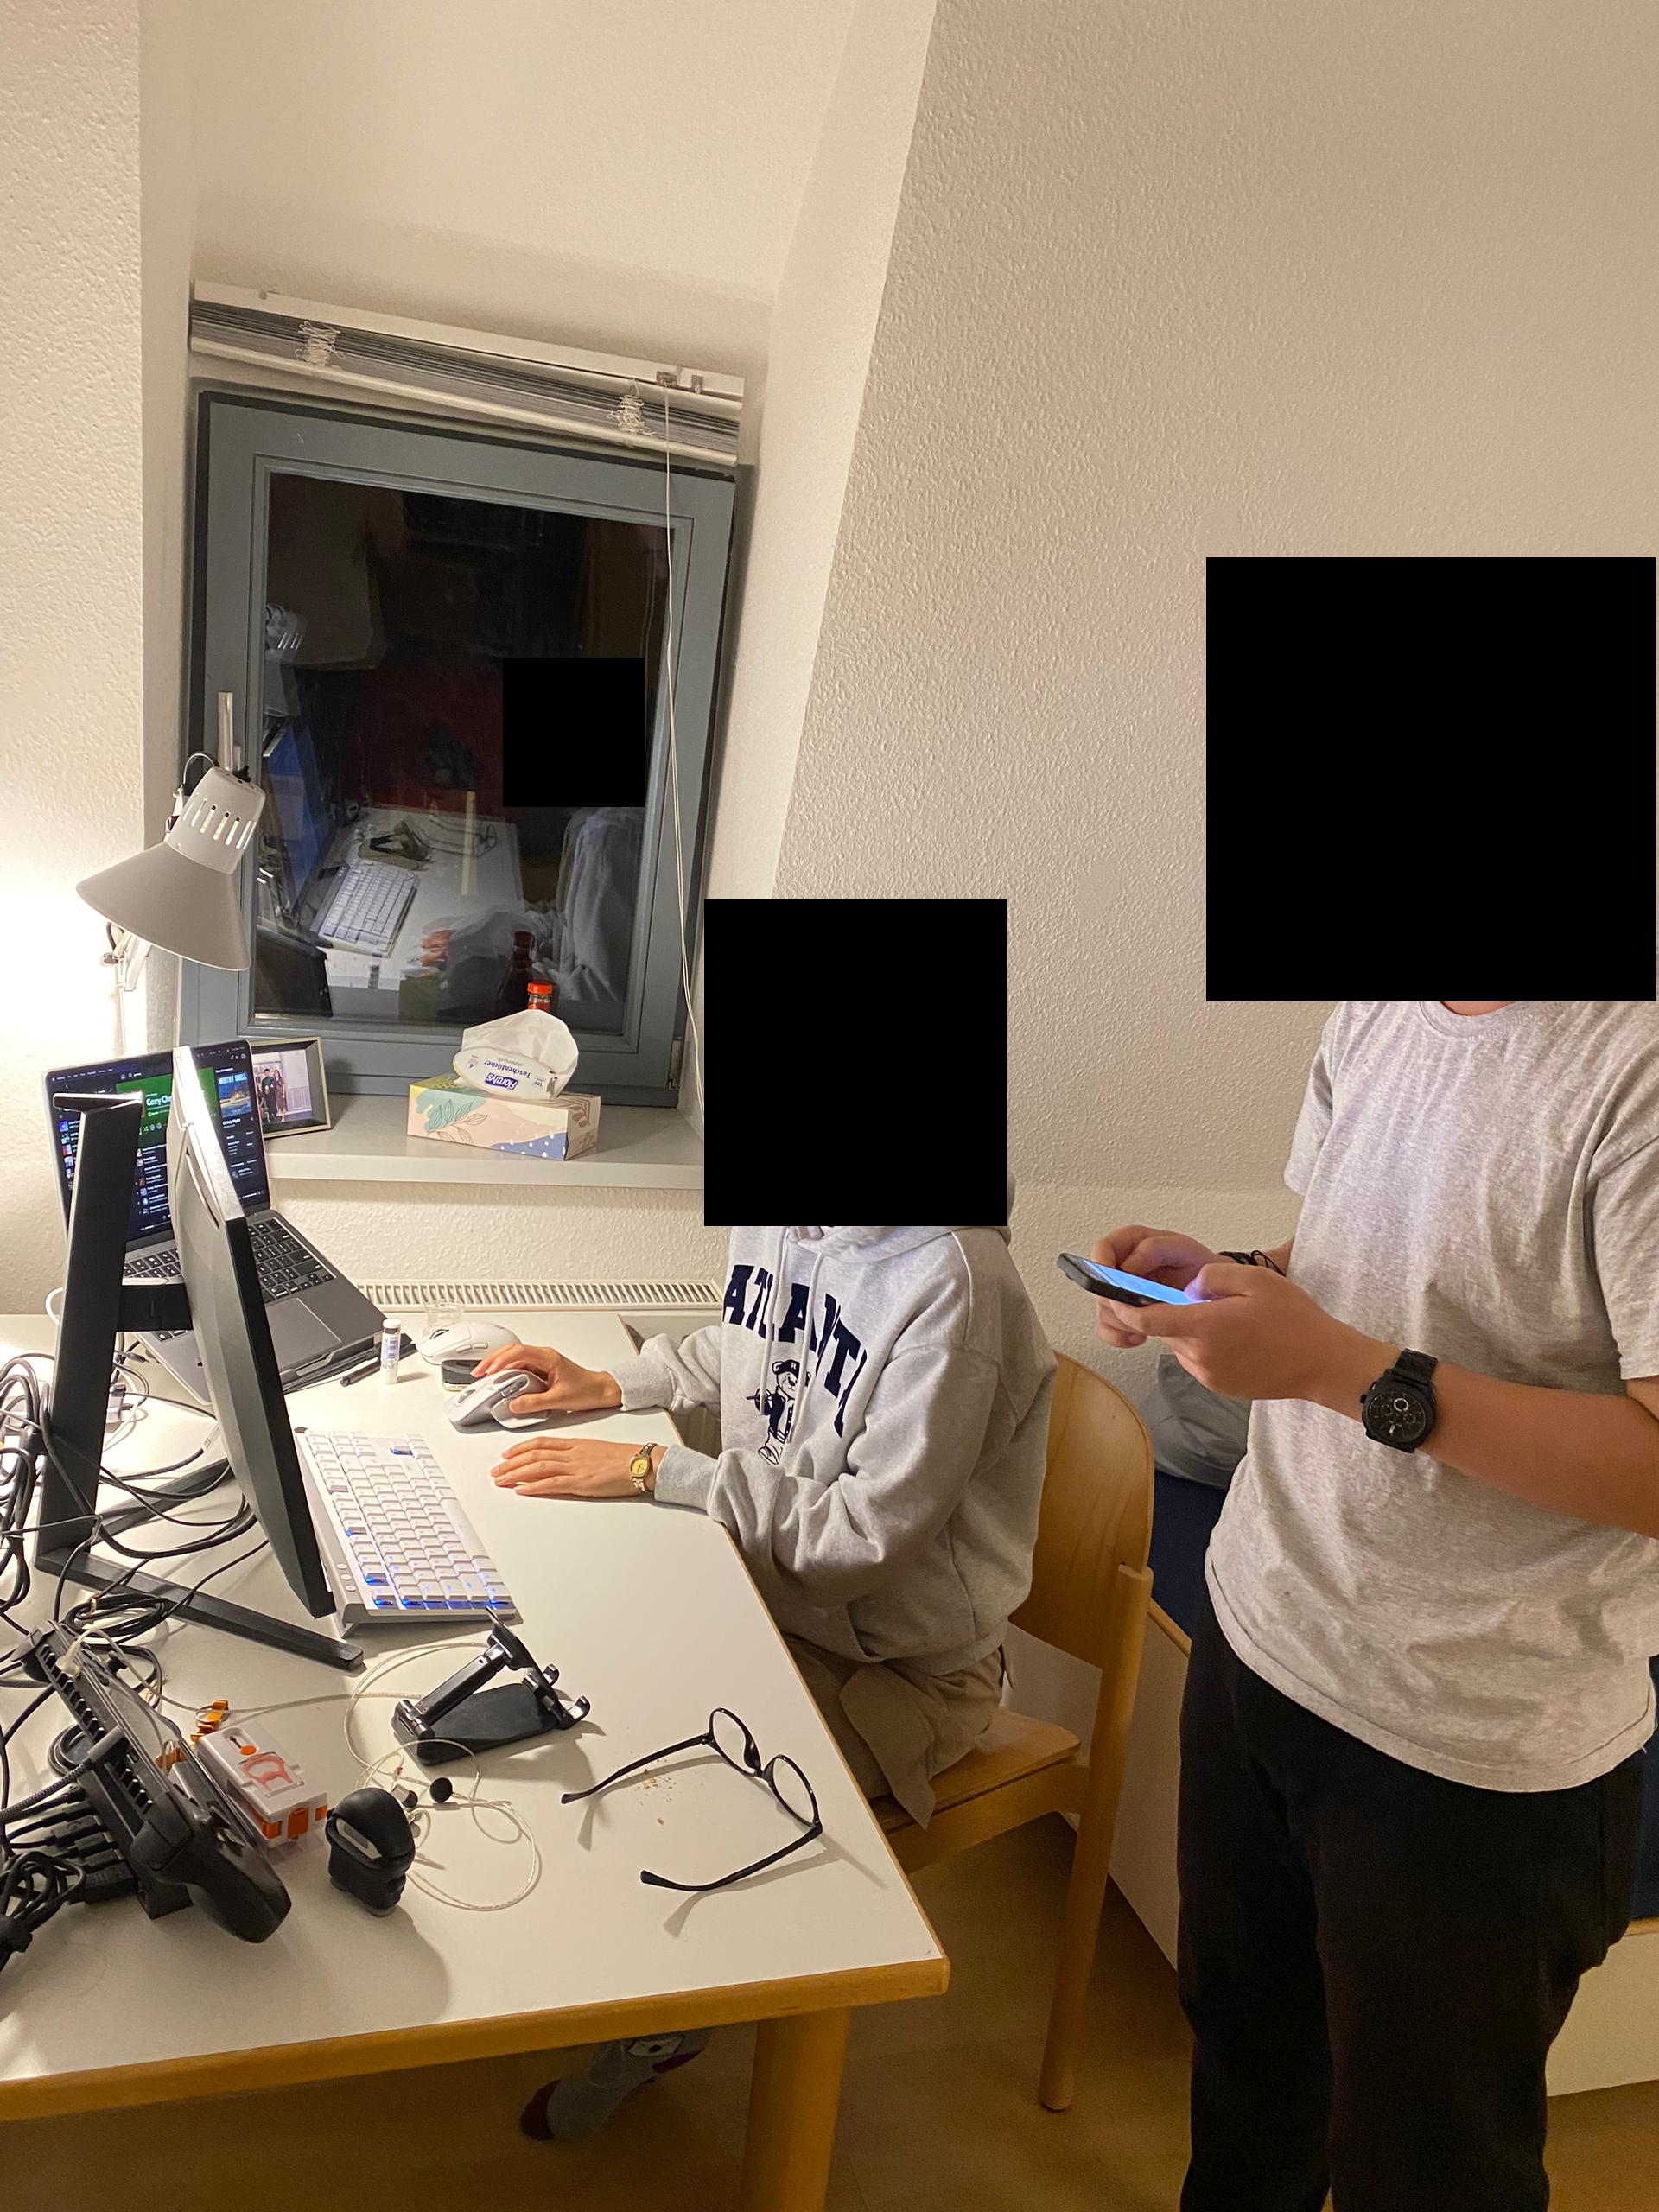
\includegraphics[width=0.5\linewidth]{Experiment.png}
    \caption{Study set-up of the experiment}
    \label{fig:placeholder}
\end{figure}




\section{Results}
Participants' reaction times varied across the two conditions. The mean reaction time of participants after mindless-scrolling indicated a slightly faster response time, with better consistency at $sd = 258.68$. The results are shown in Table~\ref{tab:rt_stats}. The descriptive statistics provides an initial overview of the effects of both conditions on cognitive performance.

\begin{table}[ht]
	\caption{Descriptive statistics for reaction time by condition (in ms)}
	\label{tab:rt_stats}
	\centering
	\begin{tabular}{lcc}
		\toprule
		Condition & Mean & SD \\
		\midrule
		Calm & 1214.18 & 370.04 \\
		Mindless & 1133.36 & 258.68 \\
		\bottomrule
	\end{tabular}
\end{table}

A paired sample t-test was performed to identify the effects of mindless-scrolling against a calm condition. The results of the t-test showed no significant difference between the mindless-scrolling and calm scenarios [$t(9) = -1.2014, p = 0.2602$]. 



To further examine on the responsiveness of participants through these conditions, we used Cohen's d to measure the effect size. The result was small to medium, with $d = -0.28$.

\section{Discussion}
The evaluation of the collected data showed that the expected reaction times under the effects of mindless-scrolling were not significant, contrary to the hypothesis. In contrast, participants react faster by $7\%$ from a mean of 1214 $ms$ to 1133 $ms$ after mindless-scrolling than at a calm state. From our observation data, the explanation may be related to our experimental design. Our experimental design consists of a 10 minute calm scenario, which was a rather monotonous session, with participants often shaking legs and fidgeting. Participants have reported that they were extremely bored and therefore began thinking about difficult topics to speed up time. This may have contributed to a slower performance, but results varied more compared to mindless-scrolling ($sd = 370$), implying that performance of participants may be affected by other conditions.

Another possible explanation was that some participants did not unmute their devices while performing the mindless-scrolling task. Playing audio alongside is common when browsing social networks. Although we did not manipulate auditory stimuli, prior research \cite{Chouhan2025, Perez2024} indicate that audio can affect reaction times. Under certain auditory conditions, the reaction times of participants decreased \cite{Perez2024}. Furthermore, the increase in audio loudness directly influences impairment in cognitive performance \cite{Laufs2024}. 

Participants performed the game task with relatively high accuracy in both conditions (mean $>85\%$), which suggests that difference in reaction time were not due to lapses during the tasks. It had also been observed that every participant struggled with the rounds near the end of the game. Therefore, this suggests that there was little flaw with the game design and that it may not have any effect in influencing the results.

\subsection{Limitations}
Due to limited time available when conducting this study, it was acknowledged that the sample size may not be adequate. However, the Cohen's $d = -0.28$ suggests that in a casual setting, there may be little benefit to reaction times between the two conditions.

The caveat of this experiment design has been outlined previously, in that the calm condition was too boring for the participants. Low-stimulus states can lead to increased internal cognitive activity, such as mind-wandering or daydreaming, which can influence reaction times \cite{Deng2022}. Participants may have engaged in these activities over the duration.

Based on the results, even though there was no significant difference, the small-to-medium effect size suggests mindless-scrolling may subtly influence the cognitive readiness. Observation on participants during the calm condition shows that fluctuating cognitive state can be a basis for the reaction time variability.

\subsection{Future Work}
The experiment conducted was small-scale with 10 participants. Future research could explore whether reaction time can be significantly larger with a larger sample size. Demographics and behaviors could also be filtered to provide an insight on the influence. Additionally, it would be valuable to examine if scrolling time and content type would influence results, particularly with negative versus neutral information. Specifically, this would be a comparison between ``doom-scrolling'' against mindless-scrolling.

\section{Conclusion}
This study identified a non-significant result between mindless-scrolling and a calming activity. This contradiction between the result and hypothesis opens questions about whether other conditions could affect reaction times. The results for this study suggests that between the two state, there was not enough evidence to suggest that the mindless-scrolling state will exhibit a significantly slower reaction time on a cognitive task as compared to the other state. It may therefore be advisable to conduct this experiment through a different direction, and avoid any tasks that can be perceived as dull for the participants.
%%
%% The acknowledgments section is defined using the "acks" environment
%% (and NOT an unnumbered section). This ensures the proper
%% identification of the section in the article metadata, and the
%% consistent spelling of the heading.
\begin{acks}
We thank the participants for giving us their time to participate in this experiment. Special recognition goes to Professor Eva and Margarita Osipova for their guidance on this research study. Pramod Bhadana helped with the ideation of this topic.
\end{acks}

%%
%% The next two lines define the bibliography style to be used, and
%% the bibliography file.
\bibliographystyle{ACM-Reference-Format}
\bibliography{main-base}


%%
%% If your work has an appendix, this is the place to put it.
\appendix

\section{Use of Large Language Models (LLMs) for Content Development}
This appendix documents the help received from Large Language Models :
\subsection{LLM for Structural Refinement(Gemini)}
\begin{itemize}
    \item \textbf{Tool/Model:} Gemini (Developed by Google)
    \item \textbf{Date of Interaction} 2025-11-08
    \item  \textbf{Purpose:} To refine the structure of the paper and word usage.
    \item \textbf{Prompt Summary:} The prompts focused on the paper's structure, specifically the method section (e.g. In both experiment conditions the subjects will play a color picking game, the condition is explained in a subsection called "Experiments Conditions" where should I explain about the game? Is this explanation repetitive?)
    \item \textbf{Outcome Summary:} The LLM suggested me to explain the game in Materials, Apparatus, or Measures, depending on what the game was used for in the study. The LLM also suggested a few fixes that can be made.
    \item \textbf{Explanation of Use:} I decided to go with the AI's suggestion and put it in the Dependent Measures subsection to show that it was used as a measuring tool. Some words were used too much (e.g. color in the game explanation) and were changed after the interaction concluded.
\end{itemize}

\subsection{LLM for Game Creation (GitHub Copilot)}
\begin{itemize}
    \item \textbf{Tool/Model:} GitHub Copilot
    \item \textbf{Date of Interaction} 2025-11-08
    \item  \textbf{Purpose:} To make the game as a measurement tool for the study.
    \item \textbf{Prompt Summary:} The prompt started with the researcher asking if they should use Client-sided rendering or Server-sided rendering to ensure the fairness of the gameplay between each participant due to the concerns of connection problem caused by the free hosting service. The LLM ended up being used to make and refine the game instead.
    \item \textbf{Outcome Summary:} After the first prompt, the LLM somehow decided to code the whole game. And after further interacting with the researcher, the LLM was used to refine the game until it satisfies the researcher.
    \item \textbf{Explanation of Use:} I had concerns that free hosting may cause connection problem while playing the game, that is what started the first prompt, after the game was automatically coded, I decided to use it to improve the game until it satisfies the whole team.
\end{itemize}
\section{Research Methods}

\subsection{Results of the Experiment}

\begin{table}[ht]
	\centering
	\caption{Reaction times (ms) for each participant under Calm and Mindless Scrolling conditions.}
	\label{tab:appendix_rt}
	\begin{tabular}{c c c}
		\toprule
		Participant & Calm (ms) & Mindless Scrolling (ms) \\
		\midrule
		1 & 1615.95 & 1235.45 \\
		2 & 841.25  & 794.55  \\
		3 & 1381.10 & 1081.95 \\
		4 & 1583.90 & 1695.40 \\
		5 & 1580.45 & 1259.35 \\
		6 & 1314.85 & 1148.50 \\
		7 & 579.75  & 780.15  \\
		8 & 721.30  & 770.55  \\
		9 & 1278.05 & 1549.55 \\
		10 & 1352.05 & 1015.65 \\
		\bottomrule
	\end{tabular}
\end{table}

\end{document}
\endinput
%%
%% End of file `sigconf-main.tex'.
